\documentclass{beamer}
\usepackage[latin1]{inputenc}
%\usetheme{Montpellier}
\usetheme{Boadilla}
%\usecolortheme[RGB={204,51,255}]{structure}
%\usecolortheme[named=purple]{structure}
\usecolortheme[RGB={62,128,62}]{structure}
%\definecolor{dark}{rgb}{0.3,0.15,0.3}
%\definecolor{light}{rgb}{0.8,0.6,0.8}
%\definecolor{reddish}{rgb}{.5,0.15,0.15}
\definecolor{dark}{rgb}{0.4,0.2,0.4}
%\definecolor{light}{rgb}{0.8,0.6,0.8}
\definecolor{reddish}{rgb}{.7,0.25,0.25}
\usepackage{graphicx}
\usepackage{pstricks}

\usepackage{tikz}
\usetikzlibrary{arrows,decorations.markings,positioning}
\usepackage{epstopdf}

\title[Mutual information for functions.]{Mutual information for functions, maybe even ERPs.}
\author{Conor Houghton}
\institute{CS, U Bristol}
\date{Frankfurt, May 2018}

\begin{document}

\maketitle



\begin{frame}{Shannon's Entropy 1}
\color{dark}
$$
H(X)=-\sum_x p(x)\log_2{p(x)}
$$
\color{black}
\end{frame}



\begin{frame}{Shannon's Entropy 2}
\color{black}
\begin{center}
\begin{tabular}{cccccccc}
1/2&1/4&1/8&1/16&1/32&1/64&1/128&1/128\\
000&001&010&011&100&101&110&111\\
0&10&110&1110&11110&111110&1111110&1111111
\end{tabular}
\end{center}
\color{dark}
$$
\mbox{average code length}=\frac{1}{2}+\frac{1}{4}2+\frac{1}{8}3+\frac{1}{16}4+\ldots = H(X)\approx 1.98 < 3
$$
\color{black}
\end{frame}


\begin{frame}{Mutual Information 1}
\color{dark}
$$
I(X,Y)=H(X)-H(X|Y)=H(Y)-H(Y|X)
$$
\color{black}
\end{frame}


\begin{frame}{Mutual Information 2}
\color{dark}
$$
I(X,Y)=\sum_{x,y} p_{X,Y}(x,y) \log_2{\frac{p_{X,Y}(x,y)}{p_X(x)p_Y(y)}}
$$
\color{black}
\end{frame}

\begin{frame}{Functions}
\color{reddish}
\begin{center}
\include{example_erps_event_sigma2}
\end{center}
\end{frame}

\begin{frame}{A dart board 1}
\color{reddish}
\begin{center}
\includegraphics[width=4cm]{dart_board.jpg}
\end{center}
\color{black}
\vfill
\color{gray}
\flushright{\small{photo from ebay (\pounds 4.20 +p.p.)}}
\color{black}
\end{frame}



\begin{frame}{A dart board 2}
\color{reddish}
\begin{center}
\includegraphics[width=4cm]{dart_board_zoom.png}
\end{center}
\color{black}
\end{frame}


\begin{frame}{Probability mass function}
\begin{center}
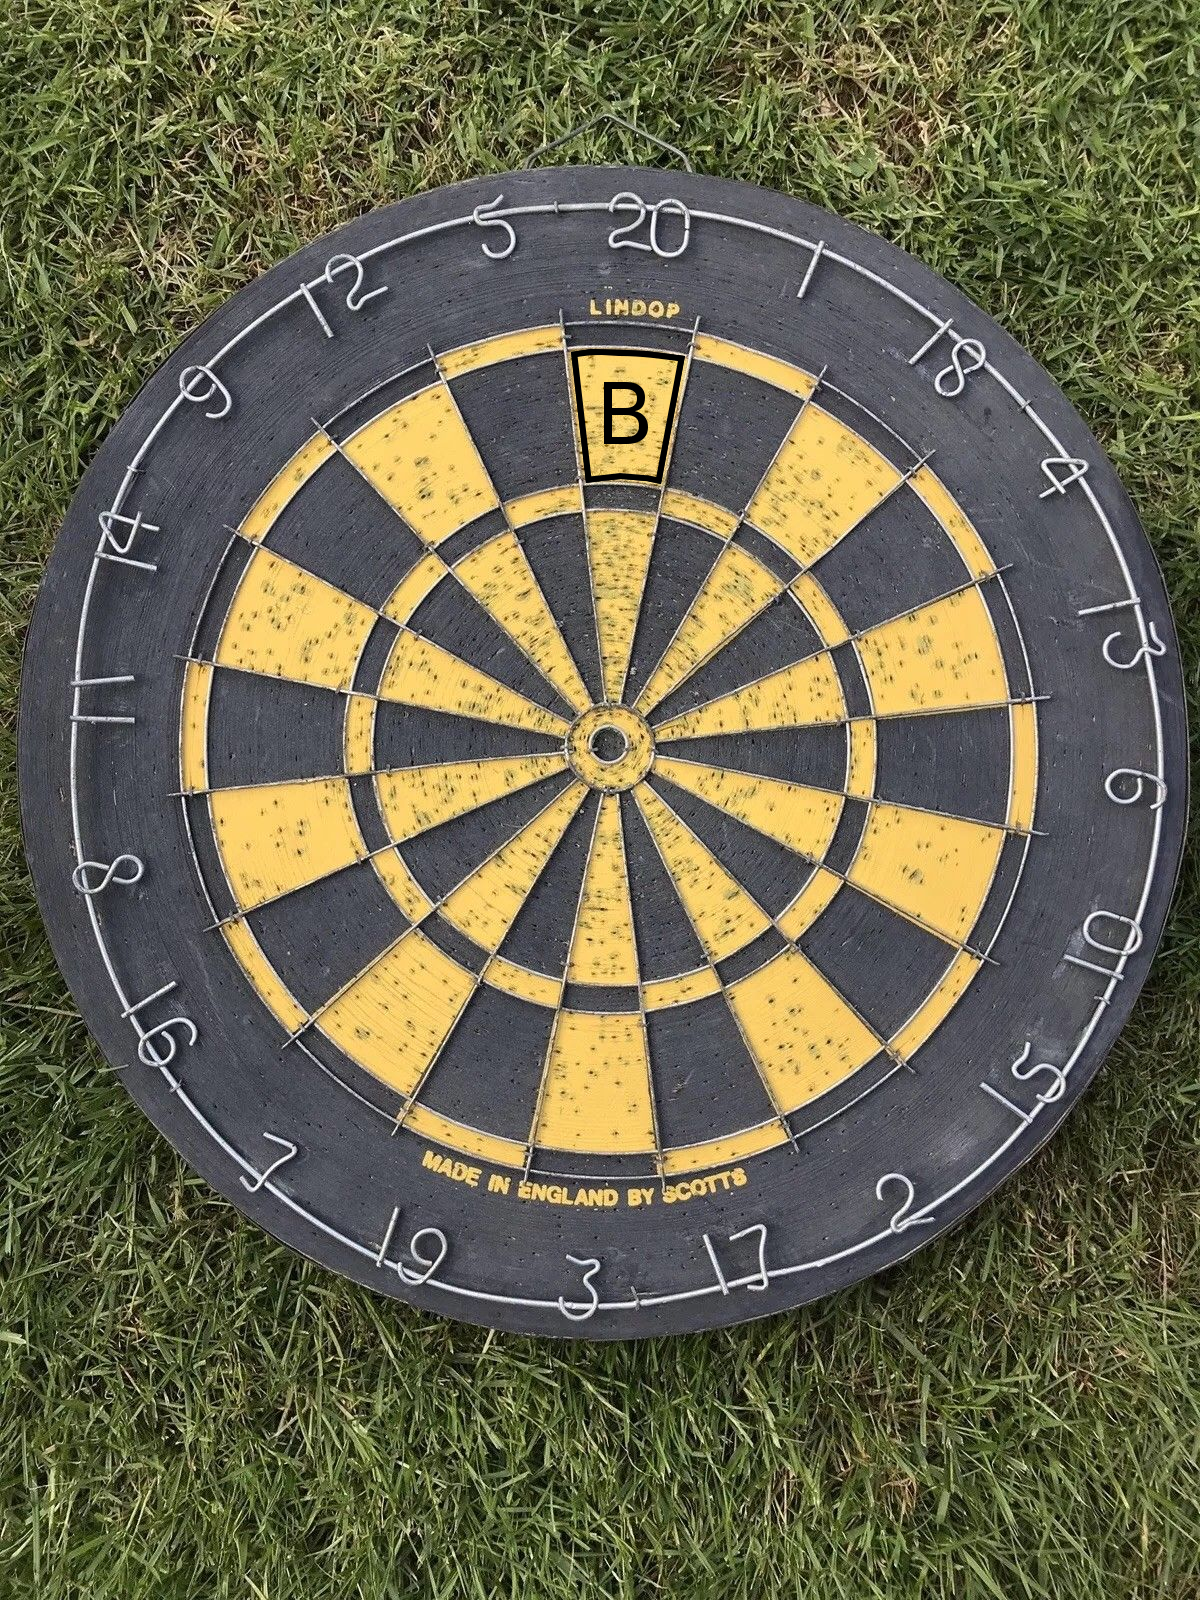
\includegraphics[width=4cm]{dart_board_region.png}
\end{center}
\color{dark}
$$\mbox{prob}(\mbox{dart lands in }B)=\int_B p(\mathbf{x})dV$$
\color{black}
\end{frame}


\begin{frame}{Estimating the number of number of holes}
\color{reddish}
\begin{center}
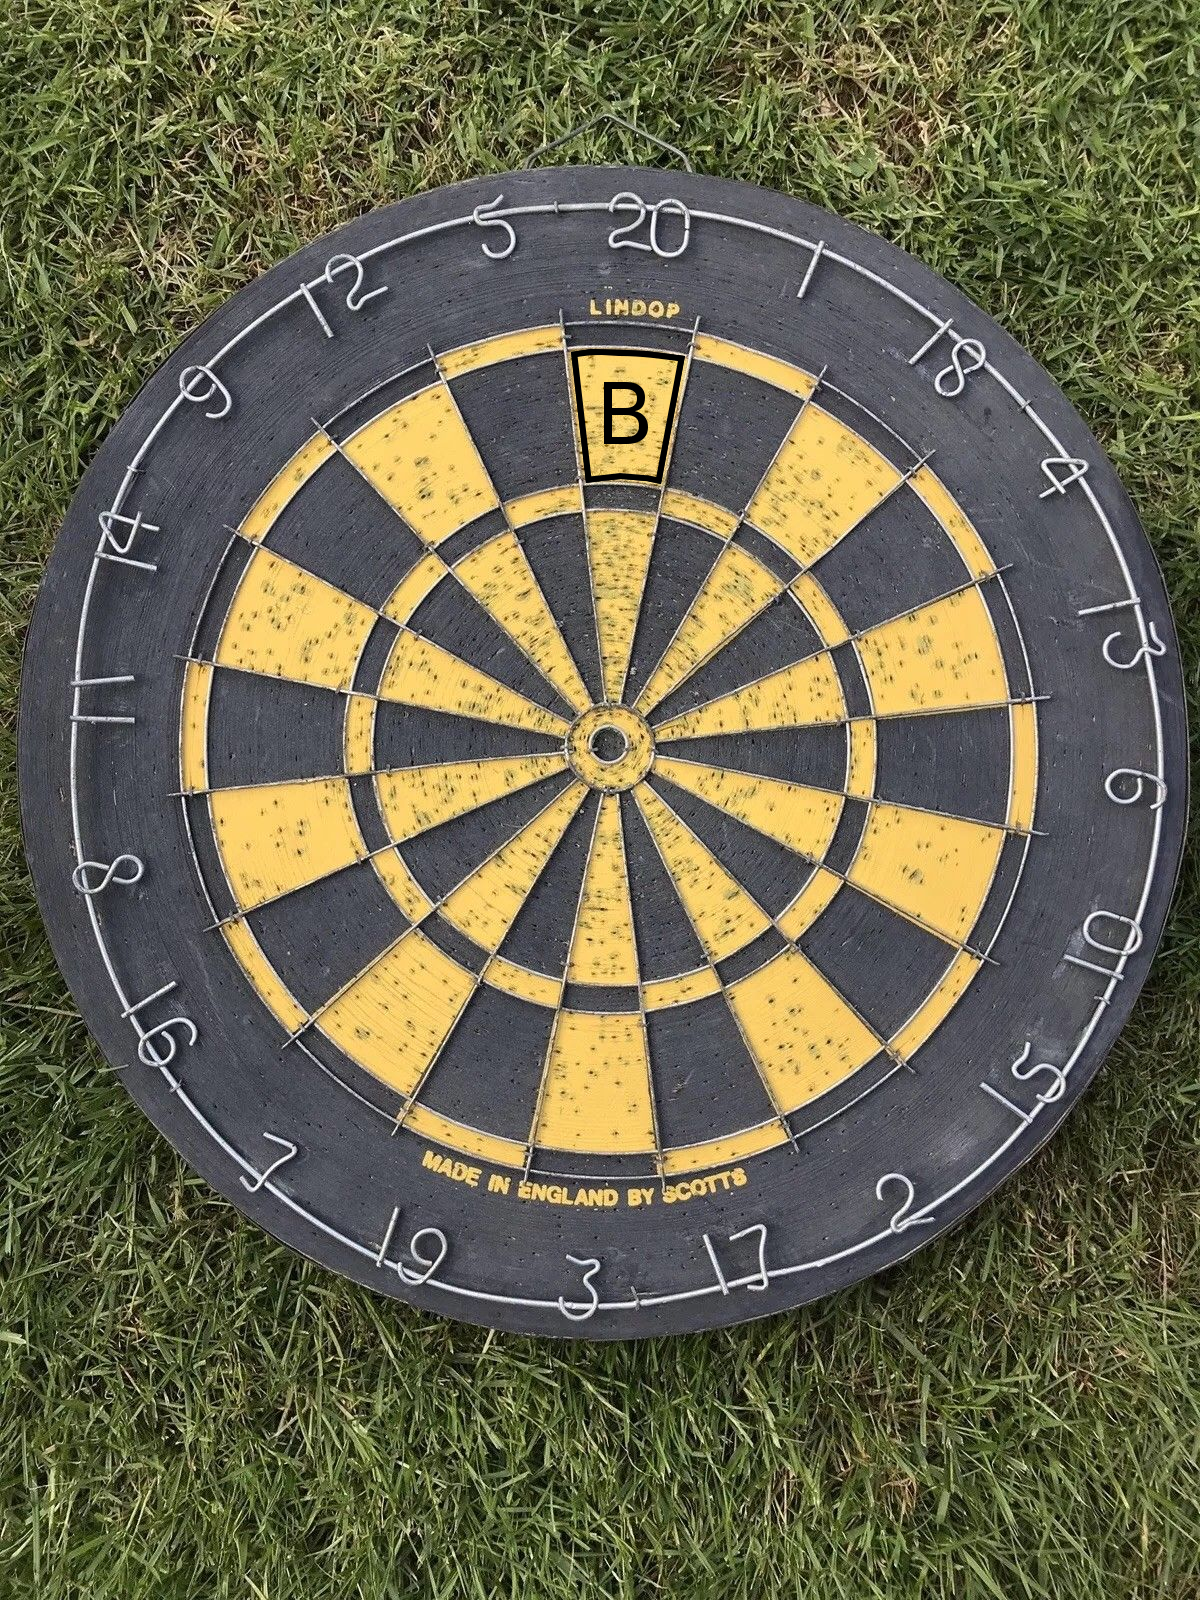
\includegraphics[width=4cm]{dart_board_region.png}
\end{center}
\color{black}
$$\langle \mbox{number of holes in }B\rangle = \int_B p(\mathbf{x})dV \times (\mbox{total number of holes})$$
\end{frame}


\begin{frame}{Estimating the probability mass function}
\color{black}
If the mass function varies slowly:
\color{dark}
$$\int_B p(\mathbf{x})dV\approx p(\mathbf{x}_0) \times \mbox{vol}\,B$$
\color{black}
so
\color{dark}
$$\mbox{number of holes in }B \approx p(\mathbf{x}_0) \times \mbox{vol}\,B \times (\mbox{total number of holes})$$
\color{black}
Using this to find the mutual information gives a \textsl{Kozachenko-Leonenko} estimator.
\end{frame}


\begin{frame}{Kozachenko-Leonenko estimators are very good}
\color{reddish}
\begin{center}
\includegraphics[width=6cm]{Birthday_Paradox.png}
\end{center}
\color{black}
\vfill
\color{gray}
\flushright{\small{graph from wikipedia article on the birthday paradox}}
\color{black}
\end{frame}



\begin{frame}{Problem}
\color{black}
How do we work out the volume in the space of functions? We have no coordinates $xyz$ to do
\color{dark}
$$\mbox{vol}\,B=\int_B dxdydz$$
\end{frame}

\begin{frame}{A dart board 3}
\color{reddish}
\begin{center}
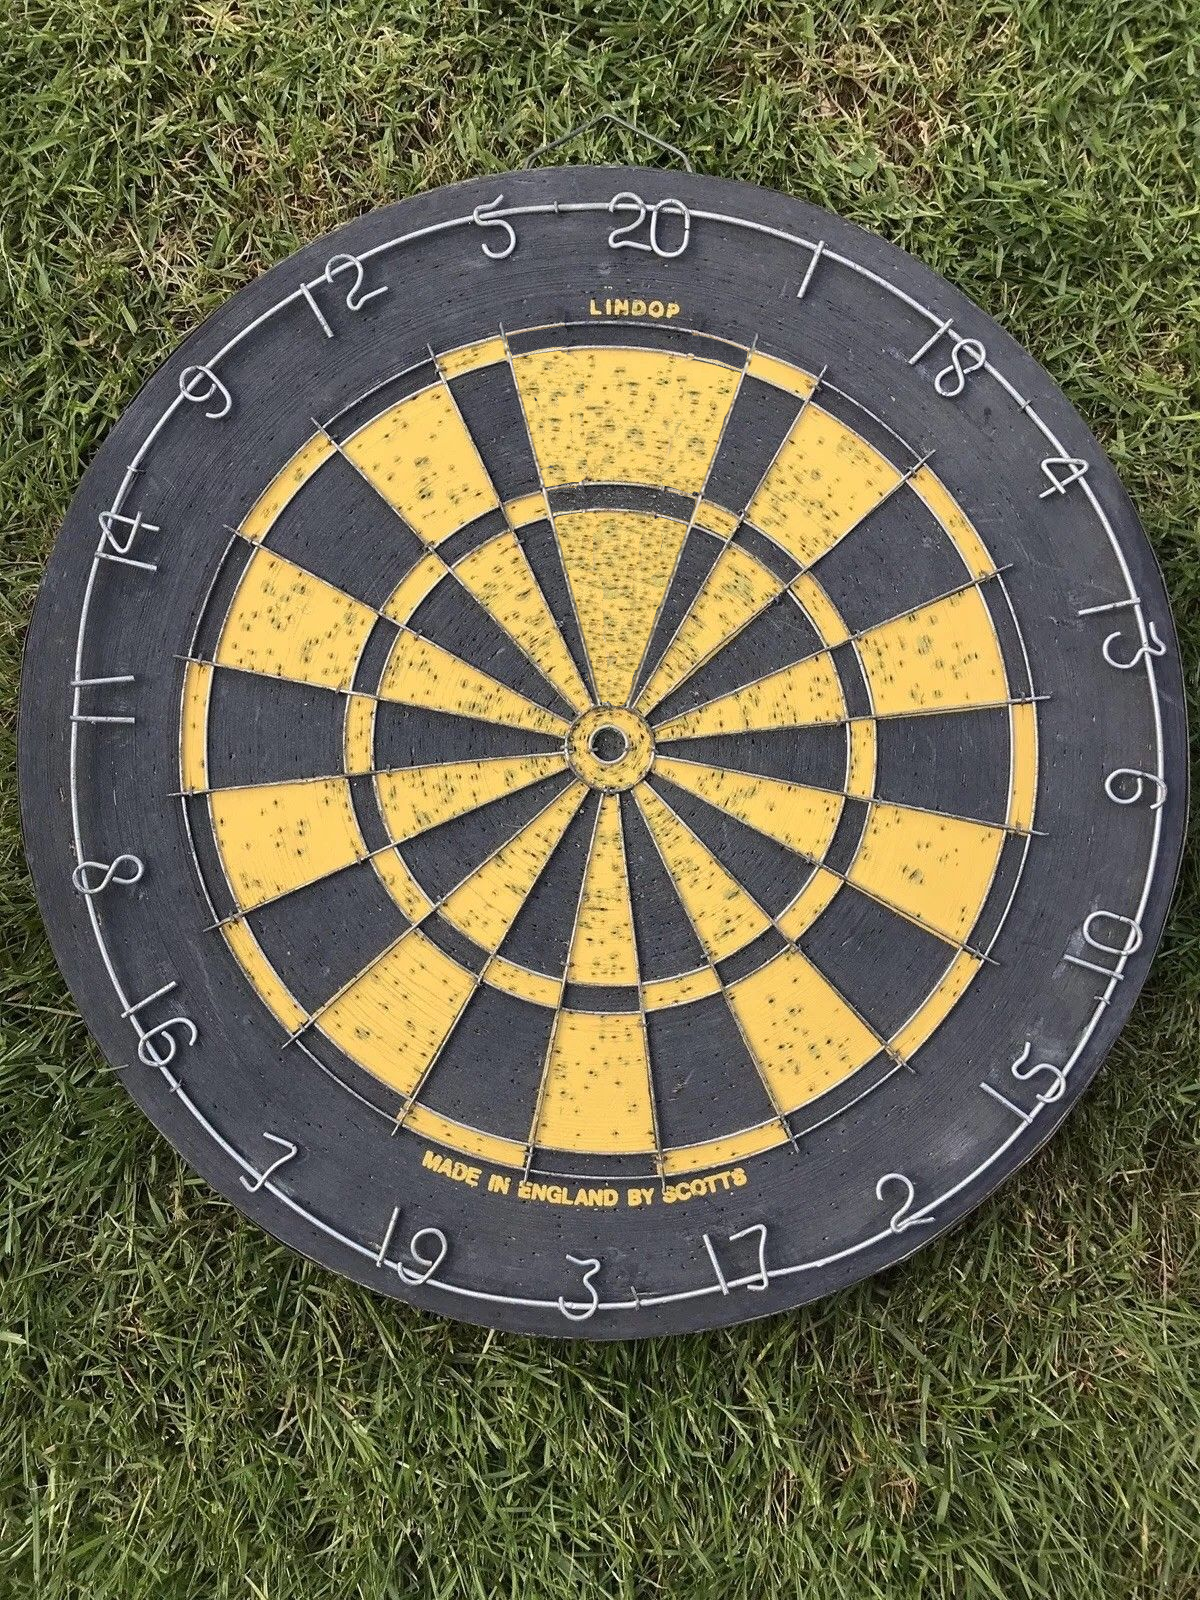
\includegraphics[width=4cm]{dart_board_big_20.png}
\end{center}
\color{dark}
$$\mbox{vol}\,B=\int_B p(\mathbf{x}) dV$$
\color{black}
\end{frame}


\begin{frame}{Volume by counting holes}
\color{dark}
$$\mbox{vol}\,B\approx \frac{\mbox{number of holes in }B}{\mbox{total number of holes}}$$
\end{frame}




\begin{frame}{Pretend ERPs 1}
\color{reddish}
\begin{center}
\include{example_erp_events}
\end{center}
\color{black} \textbf{Fictive event related potentials.} The
\lq{}stimuli\rq{} are random 5-vectors of landmarks; an ERP is
produces by perturbing the landmarks, interpolating with splines and
adding noise. \textbf{B} shows responses to different stimuli.
\color{black}
\end{frame}


\begin{frame}{Pretend ERPs 2}
\color{reddish}
\begin{center}
\include{example_erps_event_sigma0}
\end{center}
\color{black} \textbf{Multiple trials to the same stimulus.} The
amount the landmark points are moved is determined by $\sigma$; for
\textbf{A} $\sigma=0.0$, for \textbf{B} $\sigma=2$.  \color{black}
\end{frame}



\begin{frame}{Results 1}
\color{reddish}
\begin{center}
\include{info_v_event_sigma_plot}
\color{black} \textbf{Estimated mutual information.} \color{black}
\end{center}
\end{frame}


\begin{frame}{Results 2}
\color{reddish}
\begin{center}
  \include{info_v_trial_n}
\color{black} \textbf{Estimated mutual information.} Here $\sigma=1$. \color{black}
\end{center}
\end{frame}


%% \begin{frame}{Neurons}
%% \color{reddish}
%% \begin{center}
%% \includegraphics[width=6cm]{Kat_600.png}
%% \end{center}
%% \color{black}
%% \begin{center}
%% A Biocytin labelled CA1 pyramidal cell from a P14 rat hippocampus.
%% \end{center}
%% \vfill
%% \color{gray}
%% \flushright{\small{By Katarina Kolaric\\\texttt{http://www.bristol.ac.uk/neural-dynamics/programme-details/gallery}}}
%% \color{black}
%%\end{frame}

\end{document}

